\chapter{Write Away 5}

\begin{figure}[H]
    \centering
    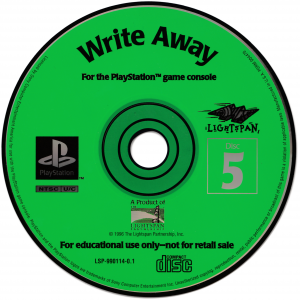
\includegraphics[width=\textwidth/2]{./Games/WriteAway/Images/WriteAway5CD.png}
    \caption{Write Away 5 CD}
\end{figure}

The fifth of the ten Write Away games published and released by The Lightspan Partnership for the PlayStation 1.

Write Away 5 features ten video programs, including an introduction video, eight story videos, and a conclusion video:

\begin{itemize}
    \item Write Away Episode Five Introduction
    \item The Lost Bear by Anna Casciari
    \item A Day in the Life of a Pioneer Girl by Katie Stall
    \item The Pets by Mark Cervero and Cory Keeler
    \item The Dream by Erika Bassaraba
    \item Baseball by Doug Shafer
    \item The Picky Pirates by Cary McTurk
    \item The Princess by Jenae Smith
    \item The Tree House by Frank Wear
    \item Write Away Conclusion
\end{itemize}

\clearpage
\newpage

\section{Transcriptions}

\subsection{The Lost Bear by Anna Casciari}

PAUL:
Okay, okay, I know we're down 50 to zero.
It's 10 below freezing out there.
All our cheerleaders have gone home.

BRIAN:
Ugh\dots

PAUL:
And we have no more sports drinks!

SCOUT, JOE:
*crying*

PAUL:
But we can do it.
Hey, why are you crying?

JOE:
I feel lost out there, coach.
I can't catch the ball.
Everyone's booing at me.
I'm a failure.

PAUL:
No, you're not a failure, you hear me?
You never failure if you go out there and you try hard.
Believe me, I know, even the littlest animal in the forest isn't a failure if he tries hard.
You can do anything you put your mind to.
You know how I know that?

BRIAN, SCOUT, JOE, SABRINA:
How coach?

PAUL:
Anna Cassiari, a first grader from Midland School, taught me this in her inspirational story, "The Lost Bear."
All right, go out there and do your best!

BRIAN, SCOUT, JOE, SABRINA:
Yeah!

BRIAN (VOICE OVER):
Once there was a bear and she just loved roses.
One day she decided to go outside to look for some roses to pick.

BABY BEAR:
Oh, how I love roses.
Their color, their fragrance.
I must have some more roses.
I know, I'll go find a rose garden and pick some for the house.

BRIAN (VOICE OVER):
But the little bear did not ask her mother for permission to go.
She just walked out the door and down the dirt path, leaving her home behind.
The little bear found some roses and she picked them.
She held the roses up to her nose and sniffed them, and suddenly she could fly high up into the sky.
Meanwhile, the mama bear realized that the little bear was gone, and she was mad.
The little bear flew over her house, and when the mama bear saw this, she said\dots

MOMA BEAR:
You come down here right now.

BRIAN (VOICE OVER):
So the little bear landed and ran to her mother.

BABY BEAR:
Here moma, I picked these flowers just for you.
And guess what, if you sniff them, you can fly!

MOMA BEAR:
Oh, well that's very nice dear, but you have done a very bad thing.
You should never leave without telling me.
For that, you must be punished.
You must stay home for 11 days and promise never to leave again without permission.

BABY BEAR:
I promise, Mama.

BRIAN (VOICE OVER):
And the little bear kept her promise and the magic roses, and they both lived happily ever after.

\subsection{A Day in the Life of a Pioneer by Katie Stall}

SABRINA:
I'm tired of practicing this ice skating.
All I do is practice.
I get up at five in the morning and practice
Then I go to school, then I come back here and practice.
This is really boring.

SCOUT (MADAM SLINKY):
To be a good skater, you must practice.
To be a good student, you must study.
Yes, to you, it may seem boring to twirl around ice in a little skirt and when you fall down, the audience goes, "eugh" but you are very lucky to be able to do so much.

SABRINA:
I guess you're right, Madam Slinky.
I have a great life with lots of friends, and I get to do all sorts of exciting things.

SCOUT (MADAM SLINKY):
Oh yes, is much better than it used to be in the old pioneer days when I was a girl.

SABRINA:
You know she's right.
I read this story about what life was really like in the pioneer days.
It comes to us from fourth grader Katie Stall, and let's all learn about a day in the life of a pioneer girl.

SCOUT (MADAM SLINKY):
And then we practice.

SABRINA:
Eugh\dots

NARRATOR:
This is a story of a pioneer girl raised in the 1800s.
Her name was Marta, and she and her family came to America from Sweden in 1852.
They settled in Wisconsin and built a farm.
They lived in a log cabin.
Marta would milk the cows and feed the chickens in the morning.
Then she and her family would have breakfast.
After breakfast, she would walk to school with her brothers.

In school, the children recited their lessons and studied arithmetic until lunchtime when they went out to play.
They would play tag, ring around the rosies, and London Bridge is Falling Down.
Then, they would walk back home to the farm and feed the animals.
Marta helped her mother bake pumpkin pies.
Then they would all eat dinner, and then go to bed.
And that's what it's like, a day in the life of a pioneer girl.
The end.

\subsection{The Pets by Mark Cervero and Cory Keeler}

BRIAN:
Alright everyone.
Today is the day we choose the new mascot for our baseball team.
Now, every team needs a good mascot to cheer them on.
Now, you're all given numbers, so let the audition begin.
Number one is um, the cheering chicken.

SABRINA (CHEERING CHICKEN):
*clucking*
Aah, oh I heard myself.

BRIAN:
Yeah, that was good.
Um, number two is the goofy gopher.
Go.

SCOUT (GOOFY GOPHER):
Oh, go team go, I can dig it, I can dig it.
Two points, two points, ten points!
Go! Go!

BRIAN:
That was a very unusual.
Uh, number three is Daryl and Daryl, the two-headed cow.

PAUL, JOE (DARYL AND DARYL):
Go, team, go, we utterly love you.
Moo.

BRIAN:
Oh, you're all very talented.
Um, now just give me a minute to think about it.
Have you ever been in a predicament like this, not knowing what animal to choose?
Making choices are always difficult, even in writing.
There are so many characters to write about, but eventually you always pick the right characters and the story turns out great.
Now, I know that's true because I just read a story that's all about choosing.
It came through right away from two authors, fourth grader Mark Cervero and kindergartener Corey Keeler of Alps Road school.
They put their heads together to come up with the perfect solution in "The Pets".

BRIAN (VOICE OVER):
Once upon a time, there lived a family.

APRIL:
Hi, I'm April, and this is my brother Crow.

CROW:
Howdy

MOTHER:
And me, I'm their mother.

BRIAN (VOICE OVER):
They were a happy family.
Now, one day, April and Crow decided to go for a walk in the forest.

MOTHER:
Be careful, kids.

BRIAN (VOICE OVER):
They walked on and on until suddenly, a ferocious bear popped out and scared the children.

BEAR:
*roar*

APRIL, CROW:
Aah!

BRIAN (VOICE OVER):
Once back home, they told their mother what they had seen.

CROW:
We saw a bear.

MOTHER:
Wait, what did this bear look like?

APRIL:
It was big and furry, and it had huge claws.

CROW:
Its breath was disgusting, it smelled like -

MOTHER:
Children, why don't you go back in the forest, catch that bear, and make him a pet?

APRIL, CROW:
Oh, mother, could we?

MOTHER:
Yes, children.

BRIAN (VOICE OVER):
So April and Crow captured the bear and made it their pet.
All went well until the bear saw toast for the first time.
He ate it all, leaving none for the family.
So they let him go.
Weeks went by, and the children were sad that they had no pet.
So April decided to go for a walk.
She found a little cat.

APRIL:
Oh, you're so cute, I'm gonna call you Little Lina.
You'll make a much better pet than a bear.

BRIAN (VOICE OVER):
Little Lena was a better pet, that is until she started throwing dead mice in the family's face.
Will the family ever get a pet?
Then Crow found a frog on the ground.

CROW:
Look, everyone, a frog will make an excellent pet!

MOTHER:
What are those bumps all over your hands?

APRIL, CROW, MOTHER:
Uh, warts!

MOTHER:
I'm sorry, children, but I don't think we'll ever find the perfect pet.

BRIAN (VOICE OVER):
Crow caught a very nice dog.

CROW:
Look, ma, a dog!

BRIAN (VOICE OVER):
The dog became the perfect pet, and they never let him go forever.

APRIL, CROW, MOTHER:
He is the perfect pet!

\subsection{The Dream by Erika Bassaraba}

SABRINA:
Next.
Very nice, next
Splended, next.
Okay, next.
What's wrong?
You have to dive in the pool like everyone else so you can't be on the team.

PAUL:
I know, but, but it's so high up here.
I can see Las Vegas.
I'm scared I might have a belly flop and hurt myself.
My bathing suit might fall down.

SABRINA:
It's scary Now, but trust me, you'll love it once you're in the water.

PAUL:
No!

SABRINA:
You know, I know a perfect poem that'll make you want to swim forever.
It comes to us from second grader Erika Bassaraba from Henry School.
You'll want to float on water once you hear "My Dream" (meant to be The Dream).

SABRINA (VOICE OVER):
I was sitting in my boat, for dessert I would make a float.
Thinking about going for a scuba dive, I wanted to catch some fish to fry.
All of a sudden, the wind began to blow, and I didn't know where my little boat would go.
I knew my life was in danger and what was about to happen was even stranger.
In the water I went, down, down, down.
I didn't know where I was being sent.
Then I saw it with my own two eyes, a big old shark was coming.
What a surprise!

I hid in the underwater sand and found a scuba diver's hand.
I unburied the scuba diver.
He looked like the Sandman who sprinkles sand in my eyes when I'm in dreamland.

WOMAN:
Then I woke up, and started to scream!
Aah!
Until I realized it was all just a dream.
Whew\dots

EVERYONE:
Come on, Paul, jump right in!

SABRINA:
See, all you have to do is try!

\subsection{Baseball by Doug Shafer}

SCOUT:
All right, now when I give you this signal *gives signal using hands* that means you throw a fastball.

JOE:
Right.

SCOUT:
All right, now, I give you this signal *gives signal using hands* you throw a curveball

JOE:
Got it?

SCOUT:
And when I do this, *gives signal using hands* that means watch out, there's a bee in your head.
All right, go out and get them, tiger!

JOE:
Oh, I can't believe it!
I'm really gonna play baseball, but there's so much to remember.
All the signals, concentration, rules of the game.
It's just like writing a story.
You have to use the rules of grammar when you write, and you have to stay really focused, or you may strike out.
I like stories that use imagery to make you feel like you're right there at the game.
Third grader Doug Shafer from Lakeview Elementary makes me feel like I'm right there behind home plate in baseball.

SON (VOICE OVER):
It was the first day of baseball.
I was up to bat, and there was one out.
It was the last inning, and it was all up to me.

DAD:
All right, son, now I know you can do it.
Don't touch my cookie.
Now I know our star hitter Slugger is injured, but the championship, not to mention my job is on the line.
Oh, and did I tell you if we lose: we'll have to move the entire franchise to Alaska?
No pressure, no pressure.
Now, go get 'em, son.

SON (VOICE OVER):
I had to hit the ball hard.
The pitcher started his wind up.
He pitched the ball, and everyone screamed.
I swung my bat and whack!
The ball flew into left field.
I was running around the bases, and [slowly to hill].
I was safe.
My coach tried to lift me up, and so did my whole team.
We won 20 to 19.
I felt so good.

DAD:
I knew you could do it son!
You're a hero!

SON:
I love this game.
Baseball, the end.

\subsection{The Picky Pirates by Cary McTurk}

PAUL:
Alright, now, remember: to stay healthy, you gotta eat from the four basic food groups.
And they are\dots

SABRINA:
Grains

BRIAN:
Dairy products

SCOUT:
Meats

JOE:
And burritos.

PAUL:
No bruiser, not burritos.
Think, think!

JOE:
Fruits and vegetables.

PAUL:
Very good.

JOE:
Yeah, very good fruit and vegetable burritos.

PAUL:
Whatever.

SCOUT:
Uh coach, uh I've been reading a lot about this eating right stuff, and I found a story that I'd like to share with all of you.
Yeah, it comes to us from Cary Mcturk, a fifth grader from Linda Vista school.
Find out what happens when you're too picky about what you eat in "The Picky Pirates."

NARRATOR:
Once upon a time, there were some pirates that sailed on a ship called the Jolly Sausage Dog.
They were very picky pirates, especially about their food.

PIRATE 1:
Arr, me [soka] is too salty!
And me ankles are swelled up!

PIRATE 2:
Arr, this fish is too fishy.
It makes my breath smell foul!

PIRATE 3:
Yes, and me soufflé is flat!

PIRATE 1, PIRATE 2, CAPTAIN:
You have a soufflé? Arr!

NARRATOR:
The captain had had enough and called for the cook.

CAPTAIN:
Cook! Cook!

COOK:
Yes captain!

CAPTAIN:
You worthless cook!
Can't you make anything we can eat?

COOK:
Well of course I can, Captain.
I can make carrots, too.
Carrot soup, carrot bread, carrots...

CAPTAIN:
Grr\dots
Walk the plank, ya swab!

NARRATOR:
Now, the little cook didn't want to die, so he tried to run away\dots but eventually, he was caught.

PIRATE 3:
I've caught him, captain.

CAPTAIN:
Yeah, you took your time.
Walk the plank.
Not you, him!
Ha ha ha.
Alright, I'm hungry, what's for supper?

PIRATE 2:
Nothing captain, we've got no cook.

NARRATOR:
Five days went by, and the pirates were starving.

PIRATE 1:
I can't go on, Captain.
I'm too hungry.

PIRATE 3:
Oh, me bellies is empty as\dots as\dots
Somebody else cook.
Can you cook?
Guess not.

NARRATOR:
Just as things looked their worst, the cook suddenly appeared.

COOK:
Captain, captain!
Here.
Here you go.
Here you go.
There you go.

CAPTAIN:
Yuck!
This tastes like slime, and it's cold.

PIRATE 3:
Oh, mine is too hot.

PIRATE 1, PIRATE 2:
Ours is just right.
Arr.

NARRATOR:
And so for five weeks, the pirates ate cold carrot soup, hot carrot soup, and just plain carrot soup.
The pirates had learned a lesson.

CAPTAIN:
Always read the resume of a cook before you hire him.
And be thankful for what you got, even if it's cold and slimy.
Eat up men!

NARRATOR:
And the pirates never complained about food again.
The end.

\subsection{The Princess by Jenae Smith}

SCOUT:
Joe.
Joe, are you listening up there?

JOE:
Yep coach.

SCOUT:
Now, now listen, Joe.
Playing center in basketball means you need to run, guard, and above all, rebound, right?

JOE:
Right!

SCOUT:
Then why won't you steal the ball?

JOE:
Because stealing's bad, coach.

SCOUT:
Yes, Joe, stealing is bad.
It hurts people.
It's not good to take what doesn't belong to you.
But when you're playing on a team, everybody gets a chance to play with the ball, right?

JOE:
Right.
But stealing the ball is bad, coach.

SCOUT:
Is there any air up there?
Uh, listen, I'm gonna tell you a story that will show you the difference between stealing, which is bad, and stealing the ball, and then you'll know what the difference is.

JOE:
I like stories.

SCOUT:
Yeah, yeah, that's good.
Listen, this story comes to us from second grader Janae Smith from Midland School.
Listen as we find out how bad stealing really can be in 'The Princess.'

SABRINA (VOICE OVER):
Once there lived a princess.
No ordinary princess.
She was pretty, smart, nice, friendly, and wonderful.
Her name was Princess Jasmine, and she lived in a castle like all princesses do.
One night while the princess was sleeping, two thieves snuck into the castle window and took all the jewels.

THIEF 1:
Help me up!
Help me up!

THIEF 2:
Alright, just be quiet.

THIEF 1:
So here we are.
Where are the Royal jewels?

THIEF 2:
In the jewelry box, you fool.
Now, there, go get 'em.
Ah, oh, look at them.
Oh, they're all belong to me, me, me.

THIEF 1:
You mean we, we, we?

THIEF 2:
Oh, whatever, let's do the dance of the jewelry theives.

THIEF 1, THIEF2:
*dance for a while*

THIEF 2:
Out of here.

SABRINA (VOICE OVER):
Soon the princess awoke.

JASMINE:
I just had the strangest dream.
I dreamed that two thieves came in that window, stole my jewels, and then danced around the room like a couple of fools.
What a silly dream.
And now, to see my jewels.
Ah, they're missing!
Father, father!

KING:
Um, yes?

JASMINE:
My jewels, I put them right in that box right before I went to bed, and now they're gone!

KING:
Oh, I told you a jewelry box wasn't safe, Jasmine.
What will you do now?

JASMINE:
The only thing a sweet, wonderful, kind, nice princess can do in a situation like this: find those two dancing fools and make them pay.

SABRINA (VOICE OVER):
Meanwhile, at the thieves' hideout:

THIEF 2:
Ten for me, one for you.
One for me, none for you.

THIEF 1:
Wait a minute!
You gave me one too many.

THIEF 2:
Ah, you're right.
With all these jewels, I'm the wealthiest man in the world, and I will take over the world.

THIEF 1:
Me too.

THIEF 2:
Oh, whatever.
Okay, let's go buy some clothes with our new ill-gotten gains.

THIEF 1:
Oh, I like it when you use big words.

SABRINA (VOICE OVER):
Princess Jasmine had followed the trail of gold from the castle to The Hideout.
She entered cautiously.

JASMINE:
Oh, there are my jewels.
I have them back.
Oh, no, the names are coming.
I must hide.

THIEF 2:
Can't believe I forgot the rest of the jewels.
Oh, they're missing.
Did you steal them?

THIEF 1:
Huh? No, I wouldn't do anything like that.

PRINCESS:
Ah ha! I've caught you both.
What you have done is terrible, almost as terrible as your dancing.
You should never steal from someone.
I was going to punish you, but if you're truly sorry, I'm sure my father can find you both jobs and you can become honest men once again.

THIEF 1, THIEF 2:
Okay.

SABRINA (VOICE OVER):
And so Princess Jasmine got her jewels back, and the thieves learned their lesson, and they all lived happily ever after.
The end.

SCOUT:
So now, Joe, do you understand the difference between stealing and stealing the ball?

JOE:
Yes.
But stealing's bad, coach.
Coach? Coach?

\subsection{The Tree House by Frank Wear}

BRIAN:
Come on!
You can do it!
All right, come on!
All right, give yourselves a hand.
Congratulations, you've just climbed the highest hill in California.
You should all be very proud of yourselves.

JOE:
Oh, we are, we are, and it's all thanks  to you.

SABRINA:
Oh, I never thought I could do anything like this.

PAUL:
Yeah, it's nice.
When do we eat?

SCOUT:
You can see for miles and miles, and look at all those stars.
Oh, it's amazing.

PAUL:
Yeah, just wonderful.
Hey, when do we eat?

SABRINA:
Oh, for goodness' sake.
Come on, everybody, let's eat.

BRIAN:
Whew.
Mountain climbing is exciting.
Not only because you use teamwork, but when you reach the top, everything takes on a different quality.
When you're way above the ground, you see everything in a different light.
A perfect example of this comes to us from first grader Frank C. Wear of Midland School.
Watch what happens when three boys enter the treehouse.

PAUL (VOICE OVER):
Once upon a time in a quiet town, there was a treehouse that three friends, Frank, Eric, and Anthony, had built.
Now, on this particular night, the three boys were in their treehouse looking out the window.

FRANK:
Nothing ever happens in this town.

ERIC:
Yes, we built this treehouse, but there's nothing exciting to see.

ANTHONY:
Hey, guys, look at that!

PAUL (VOICE OVER):
What they saw was a giant flying saucer coming right towards them.

FRANK:
You guys, I think I saw two aliens in that space!

ERIC, ANTHONY:
Yuck!

ERIC:
We must find a way to send those aliens back to Jupiter for good and save our planet.

FRANK:
I thought nothing happens in this town.

ANTHONY:
Come on, let's go!

ERIC:
Yes!

ALIEN 1:
We have landed on Earth.
Our mission is a success.

ALIEN 2:
Not yet.
Now, we must capture some earthlings and take them back to our planet for experimentation.

ALIEN 1:
And if they will not come\dots

ALIEN 2:
Then we will tickle them until they do.

ALIEN 1, ALIEN 2:
He he he. *laughing*

FRANK:
We have to build a laser beam to send them back to Jupiter.

ERIC:
Yeah, right.
How are we going to do that?

FRANK:
Well, for some time now, I've been thinking about creating a laser thing that won't hurt anybody.

ERIC:
Wow!

ANTHONY:
Okay, Mr. Smarty, how does it work?

FRANK:
Like this!

ANTHONY:
Wow!

ERIC:
Okay, Mr. Whiz Kid.
How do we use it?

FRANK:
We aim it at the spaceship and send it back to Jupiter.

PAUL (VOICE OVER):
Meanwhile, the aliens had left the spaceship to find humans.

ALIEN 1:
Why is the air so brown?

ALIEN 2:
Pollution.
They must clean up the air.

ALIEN 1:
Look, human!

ALIEN 1, ALIEN 2:
Humans!

ANTHONY:
Oh no, they saw us!

FRANK:
Quick, into the treehouse!
Come on!

ALIEN 1, ALIEN 2:
Humans!

ANTHONY:
Aah!

ALIEN 1:
Come to Jupiter with us.
Come with us, little boy.

ANTHONY:
No way!

ALIEN 2:
If you will not come with us, we will tickle you!

ANTHONY:
Noo!
*laughing*
Help!

ERIC:
Oh no, they've got Anthony.
And they're tickling him!
Oh, he's got away.

FRANK:
Oh, good.

ERIC:
He's running into their spaceship, and they're following them (should be him).
Anthony just came out.
Hit the a laser beam now Frank!

PAUL (VOICE OVER):
Frank, shot the laser beam, and the spaceship blasted up into the sky all the way back to Jupiter!

ERIC:
Yeah, it worked!

FRANK:
I told you!

ALIEN 1:
Our mission is a failure.
We have been blasted back to Jupiter.

ALIEN 2:
Not completely.
After all, Earth is a strange planet.

ALIEN 1, ALIEN 2:
Hmmmm\dots

ANTHONY:
Oh, thanks, Frank.
You saved my life.

ERIC:
Your machine was amazing.
I will never make fun of you again.

FRANK:
It was nothing, but I don't think anybody would ever believe us if we told them what we saw from our treehouse.

\subsection{Write Away Conclusion}

PAUL:
Hey, we did it you guys!
Another great show.
Thanks to all those wonderful writers out there who sent stories to us.

SCOUT:
You know, we appreciate every story you submit to us, and we read every single one of them, and it's really hard to choose what stories you're gonna see each month.

FRANK:
But we always get the job done thanks to you and a little bit of teamwork on our part.

SABRINA:
So, be a part of our team!
Keep sending us your stories, poems, and fairy tales so we can get a good workout.

JOE:
Together, we can share our talents, and our creativities, and have a really good time doing it.
Come on, everyone!
I'll race you to the next show.

PAUL:
On your mark, get set\dots

EVERYONE:
Write away!

\section{Credits}

Executive Producers: Gregg Baker, Deborah Brucher Wren, Michael Wren;
Directors: Gregg Baker, Robin LeValley;
Technical Director: Joseph S. Abreu;
Cast: Paul David, Scout Jackson, Joe Lopez, Jr., Sabrina Lu, Brian Kwan;
Writers: Deborah Brucher Wren, Robin LeValley;
Music: Rick Illes, Michael Wren;
Lighting Director: Steve Raines;
Cameras: Bill Bork, Mike Conners, Richard Crow;
Audio: Rad Corn;
Childrens Art: Blythe Baker;
Production Assistant: Sam Kephart;
Editor: Joseph S. Abreu;
Engineer: Michael Curran;
Production Coordinator: Judy Block;
Graphic Artist: Alan Scott;
Theme Song: Michael Wren;

\clearpage
\newpage

\section{Screenshots}

\begin{figure}[H]
    \centering
    \begin{subfigure}{0.45\textwidth}
        \centering
        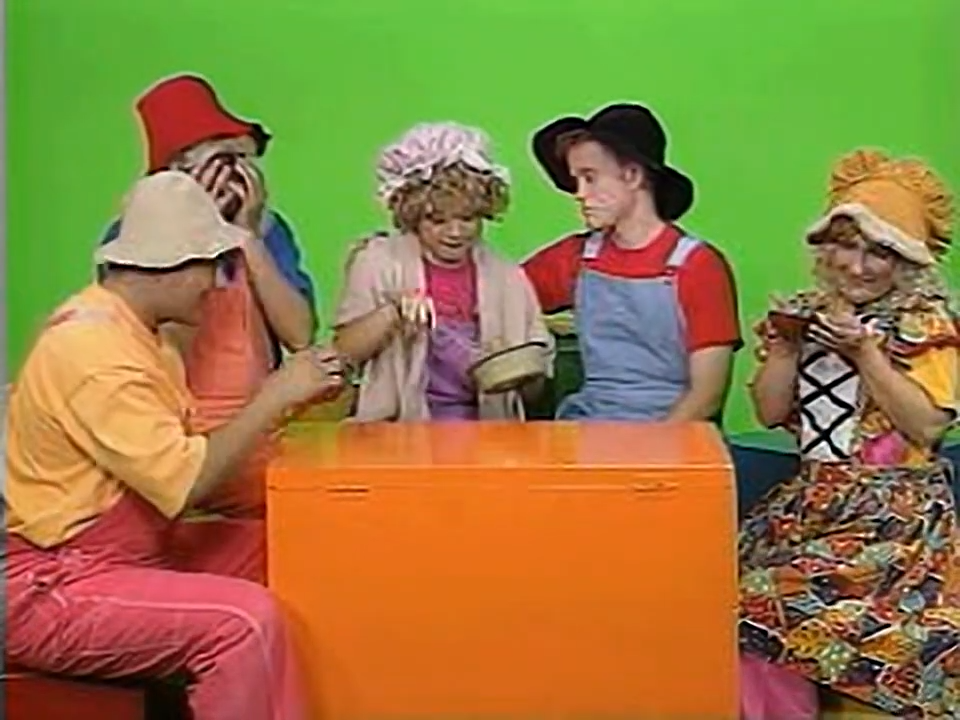
\includegraphics[width=\linewidth]{Games/WriteAway/Images/WriteAway5Screenshot1.png}
        \caption{Write Away 5 - Screenshot 1}
    \end{subfigure}
    \begin{subfigure}{0.45\textwidth}
        \centering
        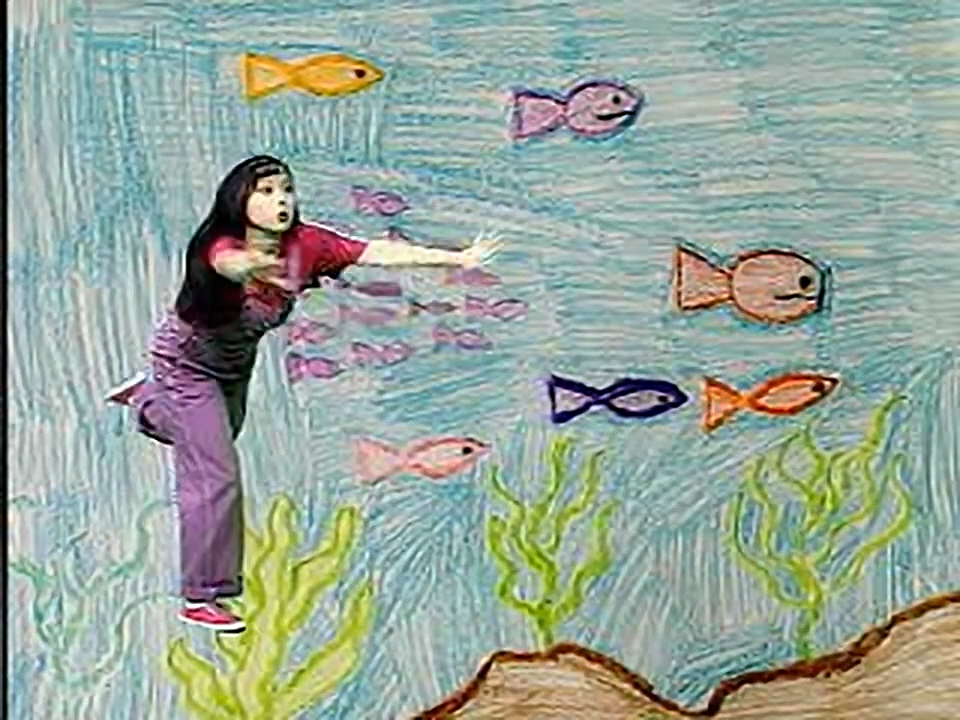
\includegraphics[width=\linewidth]{Games/WriteAway/Images/WriteAway5Screenshot2.png}
        \caption{Write Away 5 - Screenshot 2}
    \end{subfigure}

    \begin{subfigure}{0.45\textwidth}
        \centering
        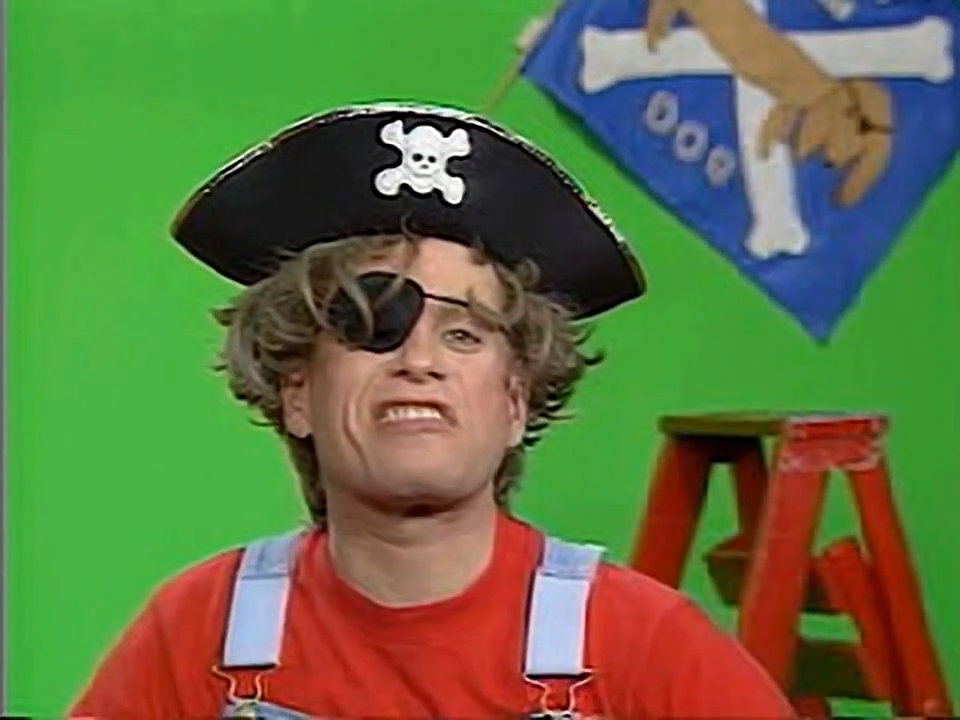
\includegraphics[width=\linewidth]{Games/WriteAway/Images/WriteAway5Screenshot3.png}
        \caption{Write Away 5 - Screenshot 3}
    \end{subfigure}
    \begin{subfigure}{0.45\textwidth}
        \centering
        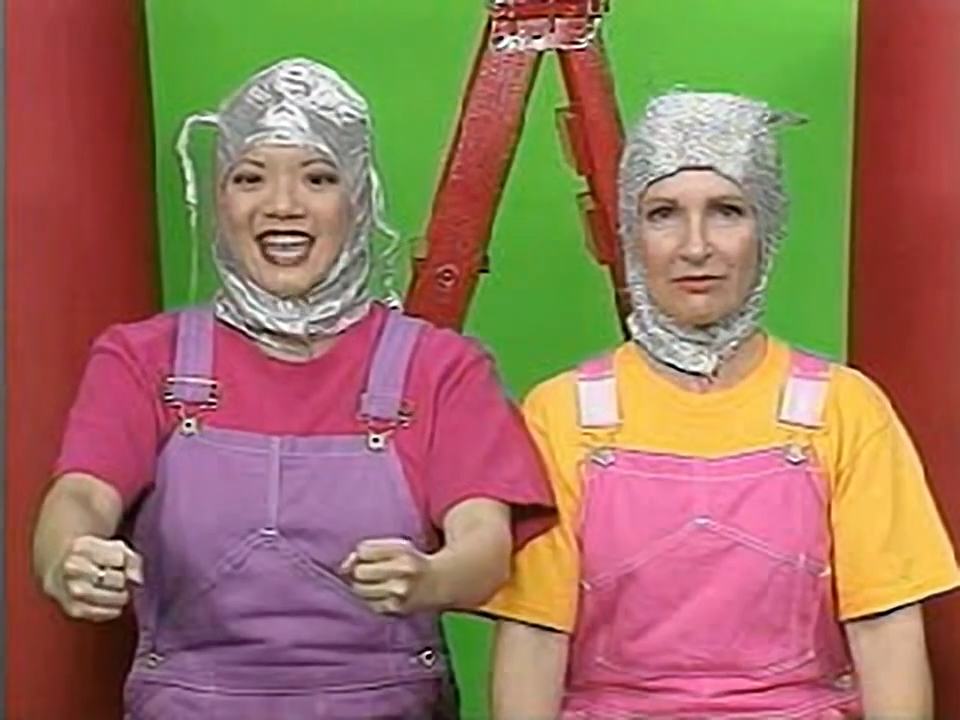
\includegraphics[width=\linewidth]{Games/WriteAway/Images/WriteAway5Screenshot4.png}
        \caption{Write Away 5 - Screenshot 4}
    \end{subfigure}
    \caption{Screenshots from Write Away 5}
\end{figure}
